\documentclass[1p]{elsarticle_modified}
%\bibliographystyle{elsarticle-num}

%\usepackage[colorlinks]{hyperref}
%\usepackage{abbrmath_seonhwa} %\Abb, \Ascr, \Acal ,\Abf, \Afrak
\usepackage{amsfonts}
\usepackage{amssymb}
\usepackage{amsmath}
\usepackage{amsthm}
\usepackage{scalefnt}
\usepackage{amsbsy}
\usepackage{kotex}
\usepackage{caption}
\usepackage{subfig}
\usepackage{color}
\usepackage{graphicx}
\usepackage{xcolor} %% white, black, red, green, blue, cyan, magenta, yellow
\usepackage{float}
\usepackage{setspace}
\usepackage{hyperref}

\usepackage{tikz}
\usetikzlibrary{arrows}

\usepackage{multirow}
\usepackage{array} % fixed length table
\usepackage{hhline}

%%%%%%%%%%%%%%%%%%%%%
\makeatletter
\renewcommand*\env@matrix[1][\arraystretch]{%
	\edef\arraystretch{#1}%
	\hskip -\arraycolsep
	\let\@ifnextchar\new@ifnextchar
	\array{*\c@MaxMatrixCols c}}
\makeatother %https://tex.stackexchange.com/questions/14071/how-can-i-increase-the-line-spacing-in-a-matrix
%%%%%%%%%%%%%%%

\usepackage[normalem]{ulem}

\newcommand{\msout}[1]{\ifmmode\text{\sout{\ensuremath{#1}}}\else\sout{#1}\fi}
%SOURCE: \msout is \stkout macro in https://tex.stackexchange.com/questions/20609/strikeout-in-math-mode

\newcommand{\cancel}[1]{
	\ifmmode
	{\color{red}\msout{#1}}
	\else
	{\color{red}\sout{#1}}
	\fi
}

\newcommand{\add}[1]{
	{\color{blue}\uwave{#1}}
}

\newcommand{\replace}[2]{
	\ifmmode
	{\color{red}\msout{#1}}{\color{blue}\uwave{#2}}
	\else
	{\color{red}\sout{#1}}{\color{blue}\uwave{#2}}
	\fi
}

\newcommand{\Sol}{\mathcal{S}} %segment
\newcommand{\D}{D} %diagram
\newcommand{\A}{\mathcal{A}} %arc


%%%%%%%%%%%%%%%%%%%%%%%%%%%%%5 test

\def\sl{\operatorname{\textup{SL}}(2,\Cbb)}
\def\psl{\operatorname{\textup{PSL}}(2,\Cbb)}
\def\quan{\mkern 1mu \triangleright \mkern 1mu}

\theoremstyle{definition}
\newtheorem{thm}{Theorem}[section]
\newtheorem{prop}[thm]{Proposition}
\newtheorem{lem}[thm]{Lemma}
\newtheorem{ques}[thm]{Question}
\newtheorem{cor}[thm]{Corollary}
\newtheorem{defn}[thm]{Definition}
\newtheorem{exam}[thm]{Example}
\newtheorem{rmk}[thm]{Remark}
\newtheorem{alg}[thm]{Algorithm}

\newcommand{\I}{\sqrt{-1}}
\begin{document}

%\begin{frontmatter}
%
%\title{Boundary parabolic representations of knots up to 8 crossings}
%
%%% Group authors per affiliation:
%\author{Yunhi Cho} 
%\address{Department of Mathematics, University of Seoul, Seoul, Korea}
%\ead{yhcho@uos.ac.kr}
%
%
%\author{Seonhwa Kim} %\fnref{s_kim}}
%\address{Center for Geometry and Physics, Institute for Basic Science, Pohang, 37673, Korea}
%\ead{ryeona17@ibs.re.kr}
%
%\author{Hyuk Kim}
%\address{Department of Mathematical Sciences, Seoul National University, Seoul 08826, Korea}
%\ead{hyukkim@snu.ac.kr}
%
%\author{Seokbeom Yoon}
%\address{Department of Mathematical Sciences, Seoul National University, Seoul, 08826,  Korea}
%\ead{sbyoon15@snu.ac.kr}
%
%\begin{abstract}
%We find all boundary parabolic representation of knots up to 8 crossings.
%
%\end{abstract}
%\begin{keyword}
%    \MSC[2010] 57M25 
%\end{keyword}
%
%\end{frontmatter}

%\linenumbers
%\tableofcontents
%
\newcommand\colored[1]{\textcolor{white}{\rule[-0.35ex]{0.8em}{1.4ex}}\kern-0.8em\color{red} #1}%
%\newcommand\colored[1]{\textcolor{white}{ #1}\kern-2.17ex	\textcolor{white}{ #1}\kern-1.81ex	\textcolor{white}{ #1}\kern-2.15ex\color{red}#1	}

{\Large $\underline{12a_{1143}~(K12a_{1143})}$}

\setlength{\tabcolsep}{10pt}
\renewcommand{\arraystretch}{1.6}
\vspace{1cm}\begin{tabular}{m{100pt}>{\centering\arraybackslash}m{274pt}}
\multirow{5}{120pt}{
	\centering
	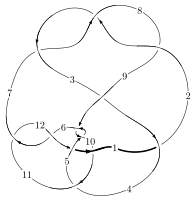
\includegraphics[width=112pt]{../../../GIT/diagram.site/Diagrams/png/1944_12a_1143.png}\\
\ \ \ A knot diagram\footnotemark}&
\allowdisplaybreaks
\textbf{Linearized knot diagam} \\
\cline{2-2}
 &
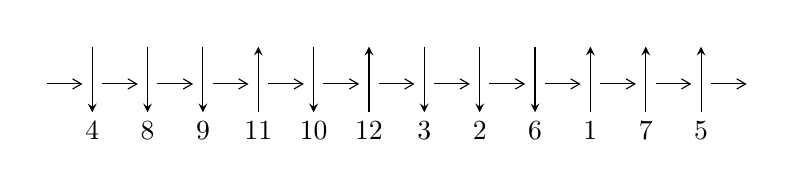
\begin{tikzpicture}[x=20pt, y=17pt]
	% nodes
	\node (C0) at (0, 0) {};
	\node (C1) at (1, 0) {};
	\node (C1U) at (1, +1) {};
	\node (C1D) at (1, -1) {4};

	\node (C2) at (2, 0) {};
	\node (C2U) at (2, +1) {};
	\node (C2D) at (2, -1) {8};

	\node (C3) at (3, 0) {};
	\node (C3U) at (3, +1) {};
	\node (C3D) at (3, -1) {9};

	\node (C4) at (4, 0) {};
	\node (C4U) at (4, +1) {};
	\node (C4D) at (4, -1) {11};

	\node (C5) at (5, 0) {};
	\node (C5U) at (5, +1) {};
	\node (C5D) at (5, -1) {10};

	\node (C6) at (6, 0) {};
	\node (C6U) at (6, +1) {};
	\node (C6D) at (6, -1) {12};

	\node (C7) at (7, 0) {};
	\node (C7U) at (7, +1) {};
	\node (C7D) at (7, -1) {3};

	\node (C8) at (8, 0) {};
	\node (C8U) at (8, +1) {};
	\node (C8D) at (8, -1) {2};

	\node (C9) at (9, 0) {};
	\node (C9U) at (9, +1) {};
	\node (C9D) at (9, -1) {6};

	\node (C10) at (10, 0) {};
	\node (C10U) at (10, +1) {};
	\node (C10D) at (10, -1) {1};

	\node (C11) at (11, 0) {};
	\node (C11U) at (11, +1) {};
	\node (C11D) at (11, -1) {7};

	\node (C12) at (12, 0) {};
	\node (C12U) at (12, +1) {};
	\node (C12D) at (12, -1) {5};
	\node (C13) at (13, 0) {};

	% arrows
	\draw[->,>={angle 60}]
	(C0) edge (C1) (C1) edge (C2) (C2) edge (C3) (C3) edge (C4) (C4) edge (C5) (C5) edge (C6) (C6) edge (C7) (C7) edge (C8) (C8) edge (C9) (C9) edge (C10) (C10) edge (C11) (C11) edge (C12) (C12) edge (C13) ;	\draw[->,>=stealth]
	(C1U) edge (C1D) (C2U) edge (C2D) (C3U) edge (C3D) (C4D) edge (C4U) (C5U) edge (C5D) (C6D) edge (C6U) (C7U) edge (C7D) (C8U) edge (C8D) (C9U) edge (C9D) (C10D) edge (C10U) (C11D) edge (C11U) (C12D) edge (C12U) ;
	\end{tikzpicture} \\
\hhline{~~} \\& 
\textbf{Solving Sequence} \\ \cline{2-2} 
 &
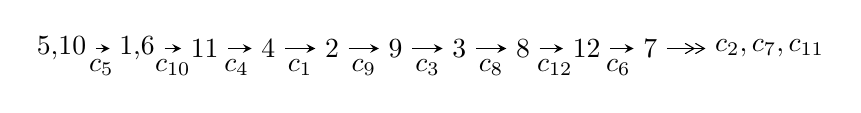
\begin{tikzpicture}[x=23pt, y=7pt]
	% node
	\node (A0) at (-1/8, 0) {5,10};
	\node (A1) at (17/16, 0) {1,6};
	\node (A2) at (17/8, 0) {11};
	\node (A3) at (25/8, 0) {4};
	\node (A4) at (33/8, 0) {2};
	\node (A5) at (41/8, 0) {9};
	\node (A6) at (49/8, 0) {3};
	\node (A7) at (57/8, 0) {8};
	\node (A8) at (65/8, 0) {12};
	\node (A9) at (73/8, 0) {7};
	\node (C1) at (1/2, -1) {$c_{5}$};
	\node (C2) at (13/8, -1) {$c_{10}$};
	\node (C3) at (21/8, -1) {$c_{4}$};
	\node (C4) at (29/8, -1) {$c_{1}$};
	\node (C5) at (37/8, -1) {$c_{9}$};
	\node (C6) at (45/8, -1) {$c_{3}$};
	\node (C7) at (53/8, -1) {$c_{8}$};
	\node (C8) at (61/8, -1) {$c_{12}$};
	\node (C9) at (69/8, -1) {$c_{6}$};
	\node (A10) at (11, 0) {$c_{2},c_{7},c_{11}$};

	% edge
	\draw[->,>=stealth]	
	(A0) edge (A1) (A1) edge (A2) (A2) edge (A3) (A3) edge (A4) (A4) edge (A5) (A5) edge (A6) (A6) edge (A7) (A7) edge (A8) (A8) edge (A9) ;
	\draw[->>,>={angle 60}]	
	(A9) edge (A10);
\end{tikzpicture} \\ 

\end{tabular} \\

\footnotetext{
The image of knot diagram is generated by the software ``\textbf{Draw programme}" developed by Andrew Bartholomew(\url{http://www.layer8.co.uk/maths/draw/index.htm\#Running-draw}), where we modified some parts for our purpose(\url{https://github.com/CATsTAILs/LinksPainter}).
}\phantom \\ \newline 
\centering \textbf{Ideals for irreducible components\footnotemark of $X_{\text{par}}$} 
 
\begin{align*}
I^u_{1}&=\langle 
-1.26077\times10^{467} u^{123}+4.32011\times10^{467} u^{122}+\cdots+2.45681\times10^{468} b+2.19615\times10^{470},\\
\phantom{I^u_{1}}&\phantom{= \langle  }9.69556\times10^{471} u^{123}-1.56547\times10^{472} u^{122}+\cdots+3.26731\times10^{472} a+4.84843\times10^{474},\\
\phantom{I^u_{1}}&\phantom{= \langle  }u^{124}-2 u^{123}+\cdots-5614 u+1364\rangle \\
I^u_{2}&=\langle 
- u^{21}- u^{20}+\cdots+b-2 u,\;-10 u^{21}-10 u^{20}+\cdots+a+1,\;u^{22}+u^{21}+\cdots+11 u^2+1\rangle \\
\\
\end{align*}
\raggedright * 2 irreducible components of $\dim_{\mathbb{C}}=0$, with total 146 representations.\\
\footnotetext{All coefficients of polynomials are rational numbers. But the coefficients are sometimes approximated in decimal forms when there is not enough margin.}
\newpage
\renewcommand{\arraystretch}{1}
\centering \section*{I. $I^u_{1}= \langle -1.26\times10^{467} u^{123}+4.32\times10^{467} u^{122}+\cdots+2.46\times10^{468} b+2.20\times10^{470},\;9.70\times10^{471} u^{123}-1.57\times10^{472} u^{122}+\cdots+3.27\times10^{472} a+4.85\times10^{474},\;u^{124}-2 u^{123}+\cdots-5614 u+1364 \rangle$}
\flushleft \textbf{(i) Arc colorings}\\
\begin{tabular}{m{7pt} m{180pt} m{7pt} m{180pt} }
\flushright $a_{5}=$&$\begin{pmatrix}1\\0\end{pmatrix}$ \\
\flushright $a_{10}=$&$\begin{pmatrix}0\\u\end{pmatrix}$ \\
\flushright $a_{1}=$&$\begin{pmatrix}-0.296744 u^{123}+0.479132 u^{122}+\cdots+78.4664 u-148.392\\0.0513172 u^{123}-0.175842 u^{122}+\cdots+506.859 u-89.3903\end{pmatrix}$ \\
\flushright $a_{6}=$&$\begin{pmatrix}1\\u^2\end{pmatrix}$ \\
\flushright $a_{11}=$&$\begin{pmatrix}0.263856 u^{123}-0.445950 u^{122}+\cdots+418.848 u-27.0755\\0.107261 u^{123}-0.307184 u^{122}+\cdots+677.350 u-134.544\end{pmatrix}$ \\
\flushright $a_{4}=$&$\begin{pmatrix}0.0329429 u^{123}+0.00314808 u^{122}+\cdots+13.4976 u-5.87222\\-0.112479 u^{123}+0.430289 u^{122}+\cdots-1616.41 u+354.133\end{pmatrix}$ \\
\flushright $a_{2}=$&$\begin{pmatrix}0.226699 u^{123}-0.407802 u^{122}+\cdots+447.589 u-58.3829\\0.0544174 u^{123}-0.110292 u^{122}+\cdots+117.960 u-7.49864\end{pmatrix}$ \\
\flushright $a_{9}=$&$\begin{pmatrix}u\\u^3+u\end{pmatrix}$ \\
\flushright $a_{3}=$&$\begin{pmatrix}0.165608 u^{123}-0.460201 u^{122}+\cdots+1639.89 u-362.844\\-0.122116 u^{123}+0.393698 u^{122}+\cdots-1282.66 u+267.260\end{pmatrix}$ \\
\flushright $a_{8}=$&$\begin{pmatrix}-0.0804638 u^{123}-0.0954324 u^{122}+\cdots+889.846 u-304.518\\0.112857 u^{123}-0.223252 u^{122}+\cdots+280.121 u-14.1022\end{pmatrix}$ \\
\flushright $a_{12}=$&$\begin{pmatrix}-0.348061 u^{123}+0.654974 u^{122}+\cdots-428.392 u-59.0017\\0.0513172 u^{123}-0.175842 u^{122}+\cdots+506.859 u-89.3903\end{pmatrix}$ \\
\flushright $a_{7}=$&$\begin{pmatrix}0.164071 u^{123}-0.393500 u^{122}+\cdots+615.316 u-105.535\\-0.0882862 u^{123}+0.0113354 u^{122}+\cdots+806.973 u-229.648\end{pmatrix}$\\&\end{tabular}
\flushleft \textbf{(ii) Obstruction class $= -1$}\\~\\
\flushleft \textbf{(iii) Cusp Shapes $= -0.298290 u^{123}+0.622766 u^{122}+\cdots-296.136 u-18.3046$}\\~\\
\newpage\renewcommand{\arraystretch}{1}
\flushleft \textbf{(iv) u-Polynomials at the component}\newline \\
\begin{tabular}{m{50pt}|m{274pt}}
Crossings & \hspace{64pt}u-Polynomials at each crossing \\
\hline $$\begin{aligned}c_{1}\end{aligned}$$&$\begin{aligned}
&u^{124}-25 u^{123}+\cdots-112353915 u+5993827
\end{aligned}$\\
\hline $$\begin{aligned}c_{2},c_{7},c_{8}\end{aligned}$$&$\begin{aligned}
&u^{124}- u^{123}+\cdots-25 u+7
\end{aligned}$\\
\hline $$\begin{aligned}c_{3}\end{aligned}$$&$\begin{aligned}
&u^{124}+u^{123}+\cdots-130387 u+20503
\end{aligned}$\\
\hline $$\begin{aligned}c_{4}\end{aligned}$$&$\begin{aligned}
&u^{124}-3 u^{122}+\cdots+161 u+13
\end{aligned}$\\
\hline $$\begin{aligned}c_{5},c_{9}\end{aligned}$$&$\begin{aligned}
&u^{124}+2 u^{123}+\cdots+5614 u+1364
\end{aligned}$\\
\hline $$\begin{aligned}c_{6},c_{11}\end{aligned}$$&$\begin{aligned}
&u^{124}+u^{123}+\cdots+23 u^2+1
\end{aligned}$\\
\hline $$\begin{aligned}c_{10}\end{aligned}$$&$\begin{aligned}
&u^{124}+15 u^{123}+\cdots+55987 u+6721
\end{aligned}$\\
\hline $$\begin{aligned}c_{12}\end{aligned}$$&$\begin{aligned}
&u^{124}-7 u^{123}+\cdots+4 u+5
\end{aligned}$\\
\hline
\end{tabular}\\~\\
\newpage\renewcommand{\arraystretch}{1}
\flushleft \textbf{(v) Riley Polynomials at the component}\newline \\
\begin{tabular}{m{50pt}|m{274pt}}
Crossings & \hspace{64pt}Riley Polynomials at each crossing \\
\hline $$\begin{aligned}c_{1}\end{aligned}$$&$\begin{aligned}
&y^{124}+63 y^{123}+\cdots+431798753106101 y+35925962105929
\end{aligned}$\\
\hline $$\begin{aligned}c_{2},c_{7},c_{8}\end{aligned}$$&$\begin{aligned}
&y^{124}+115 y^{123}+\cdots-611 y+49
\end{aligned}$\\
\hline $$\begin{aligned}c_{3}\end{aligned}$$&$\begin{aligned}
&y^{124}+21 y^{123}+\cdots+4053965961 y+420373009
\end{aligned}$\\
\hline $$\begin{aligned}c_{4}\end{aligned}$$&$\begin{aligned}
&y^{124}-6 y^{123}+\cdots-1091 y+169
\end{aligned}$\\
\hline $$\begin{aligned}c_{5},c_{9}\end{aligned}$$&$\begin{aligned}
&y^{124}+84 y^{123}+\cdots+69263508 y+1860496
\end{aligned}$\\
\hline $$\begin{aligned}c_{6},c_{11}\end{aligned}$$&$\begin{aligned}
&y^{124}+75 y^{123}+\cdots+46 y+1
\end{aligned}$\\
\hline $$\begin{aligned}c_{10}\end{aligned}$$&$\begin{aligned}
&y^{124}-39 y^{123}+\cdots+13491579 y+45171841
\end{aligned}$\\
\hline $$\begin{aligned}c_{12}\end{aligned}$$&$\begin{aligned}
&y^{124}-9 y^{123}+\cdots+764 y+25
\end{aligned}$\\
\hline
\end{tabular}\\~\\
\newpage\flushleft \textbf{(vi) Complex Volumes and Cusp Shapes}
$$\begin{array}{c|c|c}  
\text{Solutions to }I^u_{1}& \I (\text{vol} + \sqrt{-1}CS) & \text{Cusp shape}\\
 \hline 
\begin{aligned}
u &= -0.429038 + 0.902009 I \\
a &= \phantom{-}1.68525 - 0.38916 I \\
b &= -0.311918 - 0.444710 I\end{aligned}
 & -1.32425 + 6.17844 I & \phantom{-0.000000 } 0 \\ \hline\begin{aligned}
u &= -0.429038 - 0.902009 I \\
a &= \phantom{-}1.68525 + 0.38916 I \\
b &= -0.311918 + 0.444710 I\end{aligned}
 & -1.32425 - 6.17844 I & \phantom{-0.000000 } 0 \\ \hline\begin{aligned}
u &= \phantom{-}0.462532 + 0.888982 I \\
a &= -1.76445 - 0.60323 I \\
b &= \phantom{-}0.303288 - 0.490179 I\end{aligned}
 & \phantom{-}4.02276 - 9.56251 I & \phantom{-0.000000 } 0 \\ \hline\begin{aligned}
u &= \phantom{-}0.462532 - 0.888982 I \\
a &= -1.76445 + 0.60323 I \\
b &= \phantom{-}0.303288 + 0.490179 I\end{aligned}
 & \phantom{-}4.02276 + 9.56251 I & \phantom{-0.000000 } 0 \\ \hline\begin{aligned}
u &= -0.700036 + 0.709979 I \\
a &= \phantom{-}0.229510 + 0.746472 I \\
b &= \phantom{-}0.124354 + 0.576117 I\end{aligned}
 & \phantom{-}3.94855 + 2.83097 I & \phantom{-0.000000 } 0 \\ \hline\begin{aligned}
u &= -0.700036 - 0.709979 I \\
a &= \phantom{-}0.229510 - 0.746472 I \\
b &= \phantom{-}0.124354 - 0.576117 I\end{aligned}
 & \phantom{-}3.94855 - 2.83097 I & \phantom{-0.000000 } 0 \\ \hline\begin{aligned}
u &= \phantom{-}0.981319 + 0.236471 I \\
a &= -0.783751 - 0.565134 I \\
b &= -0.617900 - 0.966488 I\end{aligned}
 & -2.59935 + 5.08228 I & \phantom{-0.000000 } 0 \\ \hline\begin{aligned}
u &= \phantom{-}0.981319 - 0.236471 I \\
a &= -0.783751 + 0.565134 I \\
b &= -0.617900 + 0.966488 I\end{aligned}
 & -2.59935 - 5.08228 I & \phantom{-0.000000 } 0 \\ \hline\begin{aligned}
u &= \phantom{-}0.086681 + 0.973158 I \\
a &= -0.00243 + 1.90093 I \\
b &= \phantom{-}0.030909 + 1.238560 I\end{aligned}
 & \phantom{-}2.62831 - 4.26746 I & \phantom{-0.000000 } 0 \\ \hline\begin{aligned}
u &= \phantom{-}0.086681 - 0.973158 I \\
a &= -0.00243 - 1.90093 I \\
b &= \phantom{-}0.030909 - 1.238560 I\end{aligned}
 & \phantom{-}2.62831 + 4.26746 I & \phantom{-0.000000 } 0\\
 \hline 
 \end{array}$$\newpage$$\begin{array}{c|c|c}  
\text{Solutions to }I^u_{1}& \I (\text{vol} + \sqrt{-1}CS) & \text{Cusp shape}\\
 \hline 
\begin{aligned}
u &= \phantom{-}0.095969 + 1.021210 I \\
a &= \phantom{-}0.220373 - 0.630602 I \\
b &= -1.72011 - 1.08206 I\end{aligned}
 & \phantom{-}2.69663 - 0.68082 I & \phantom{-0.000000 } 0 \\ \hline\begin{aligned}
u &= \phantom{-}0.095969 - 1.021210 I \\
a &= \phantom{-}0.220373 + 0.630602 I \\
b &= -1.72011 + 1.08206 I\end{aligned}
 & \phantom{-}2.69663 + 0.68082 I & \phantom{-0.000000 } 0 \\ \hline\begin{aligned}
u &= \phantom{-}0.370950 + 0.971281 I \\
a &= -1.241830 - 0.070439 I \\
b &= \phantom{-}0.371399 - 0.335424 I\end{aligned}
 & \phantom{-}0.09413 - 2.84309 I & \phantom{-0.000000 } 0 \\ \hline\begin{aligned}
u &= \phantom{-}0.370950 - 0.971281 I \\
a &= -1.241830 + 0.070439 I \\
b &= \phantom{-}0.371399 + 0.335424 I\end{aligned}
 & \phantom{-}0.09413 + 2.84309 I & \phantom{-0.000000 } 0 \\ \hline\begin{aligned}
u &= \phantom{-}0.313151 + 0.906275 I \\
a &= -1.54848 + 0.35133 I \\
b &= \phantom{-}0.262555 - 0.312852 I\end{aligned}
 & \phantom{-}0.11097 - 3.14486 I & \phantom{-0.000000 } 0 \\ \hline\begin{aligned}
u &= \phantom{-}0.313151 - 0.906275 I \\
a &= -1.54848 - 0.35133 I \\
b &= \phantom{-}0.262555 + 0.312852 I\end{aligned}
 & \phantom{-}0.11097 + 3.14486 I & \phantom{-0.000000 } 0 \\ \hline\begin{aligned}
u &= -0.164015 + 1.040220 I \\
a &= -0.054409 - 0.616648 I \\
b &= \phantom{-}1.58232 - 1.32724 I\end{aligned}
 & \phantom{-}1.24453 + 5.17092 I & \phantom{-0.000000 } 0 \\ \hline\begin{aligned}
u &= -0.164015 - 1.040220 I \\
a &= -0.054409 + 0.616648 I \\
b &= \phantom{-}1.58232 + 1.32724 I\end{aligned}
 & \phantom{-}1.24453 - 5.17092 I & \phantom{-0.000000 } 0 \\ \hline\begin{aligned}
u &= -0.212093 + 0.914220 I \\
a &= \phantom{-}1.20372 + 0.90772 I \\
b &= -0.201605 - 0.220439 I\end{aligned}
 & -2.33446 + 0.04536 I & \phantom{-0.000000 } 0 \\ \hline\begin{aligned}
u &= -0.212093 - 0.914220 I \\
a &= \phantom{-}1.20372 - 0.90772 I \\
b &= -0.201605 + 0.220439 I\end{aligned}
 & -2.33446 - 0.04536 I & \phantom{-0.000000 } 0\\
 \hline 
 \end{array}$$\newpage$$\begin{array}{c|c|c}  
\text{Solutions to }I^u_{1}& \I (\text{vol} + \sqrt{-1}CS) & \text{Cusp shape}\\
 \hline 
\begin{aligned}
u &= -0.804822 + 0.421468 I \\
a &= -0.378791 - 1.325140 I \\
b &= -0.884556 - 0.459821 I\end{aligned}
 & \phantom{-}5.66189 + 7.24435 I & \phantom{-0.000000 } 0 \\ \hline\begin{aligned}
u &= -0.804822 - 0.421468 I \\
a &= -0.378791 + 1.325140 I \\
b &= -0.884556 + 0.459821 I\end{aligned}
 & \phantom{-}5.66189 - 7.24435 I & \phantom{-0.000000 } 0 \\ \hline\begin{aligned}
u &= \phantom{-}0.198160 + 1.075310 I \\
a &= -0.017029 - 0.668357 I \\
b &= -1.45606 - 1.33338 I\end{aligned}
 & \phantom{-}6.92773 - 9.08534 I & \phantom{-0.000000 } 0 \\ \hline\begin{aligned}
u &= \phantom{-}0.198160 - 1.075310 I \\
a &= -0.017029 + 0.668357 I \\
b &= -1.45606 + 1.33338 I\end{aligned}
 & \phantom{-}6.92773 + 9.08534 I & \phantom{-0.000000 } 0 \\ \hline\begin{aligned}
u &= \phantom{-}0.148724 + 0.891560 I \\
a &= -1.00500 + 1.31466 I \\
b &= \phantom{-}0.137345 - 0.196084 I\end{aligned}
 & \phantom{-}2.53652 + 3.22819 I & \phantom{-0.000000 } 0 \\ \hline\begin{aligned}
u &= \phantom{-}0.148724 - 0.891560 I \\
a &= -1.00500 - 1.31466 I \\
b &= \phantom{-}0.137345 + 0.196084 I\end{aligned}
 & \phantom{-}2.53652 - 3.22819 I & \phantom{-0.000000 } 0 \\ \hline\begin{aligned}
u &= -0.086394 + 0.891345 I \\
a &= \phantom{-}0.01279 + 1.90669 I \\
b &= -0.028215 + 1.210280 I\end{aligned}
 & -2.79053 + 1.40664 I & \phantom{-0.000000 } 0 \\ \hline\begin{aligned}
u &= -0.086394 - 0.891345 I \\
a &= \phantom{-}0.01279 - 1.90669 I \\
b &= -0.028215 - 1.210280 I\end{aligned}
 & -2.79053 - 1.40664 I & \phantom{-0.000000 } 0 \\ \hline\begin{aligned}
u &= \phantom{-}0.022631 + 0.891353 I \\
a &= \phantom{-}0.678765 - 0.708120 I \\
b &= -1.63314 - 0.40873 I\end{aligned}
 & \phantom{-}2.07163 + 0.00309 I & \phantom{-0.000000 } 0 \\ \hline\begin{aligned}
u &= \phantom{-}0.022631 - 0.891353 I \\
a &= \phantom{-}0.678765 + 0.708120 I \\
b &= -1.63314 + 0.40873 I\end{aligned}
 & \phantom{-}2.07163 - 0.00309 I & \phantom{-0.000000 } 0\\
 \hline 
 \end{array}$$\newpage$$\begin{array}{c|c|c}  
\text{Solutions to }I^u_{1}& \I (\text{vol} + \sqrt{-1}CS) & \text{Cusp shape}\\
 \hline 
\begin{aligned}
u &= \phantom{-}0.585165 + 0.655216 I \\
a &= -0.02505 + 1.56182 I \\
b &= \phantom{-}0.197316 + 1.012240 I\end{aligned}
 & \phantom{-}3.36567 + 5.34298 I & \phantom{-0.000000 } 0 \\ \hline\begin{aligned}
u &= \phantom{-}0.585165 - 0.655216 I \\
a &= -0.02505 - 1.56182 I \\
b &= \phantom{-}0.197316 - 1.012240 I\end{aligned}
 & \phantom{-}3.36567 - 5.34298 I & \phantom{-0.000000 } 0 \\ \hline\begin{aligned}
u &= -0.500010 + 1.005970 I \\
a &= \phantom{-}1.076970 - 0.838445 I \\
b &= -0.498140 - 0.541028 I\end{aligned}
 & \phantom{-}5.50091 + 1.31479 I & \phantom{-0.000000 } 0 \\ \hline\begin{aligned}
u &= -0.500010 - 1.005970 I \\
a &= \phantom{-}1.076970 + 0.838445 I \\
b &= -0.498140 + 0.541028 I\end{aligned}
 & \phantom{-}5.50091 - 1.31479 I & \phantom{-0.000000 } 0 \\ \hline\begin{aligned}
u &= -0.027819 + 1.125170 I \\
a &= -0.189806 - 0.869996 I \\
b &= \phantom{-}1.39218 - 1.00783 I\end{aligned}
 & \phantom{-}9.87166 - 0.88998 I & \phantom{-0.000000 } 0 \\ \hline\begin{aligned}
u &= -0.027819 - 1.125170 I \\
a &= -0.189806 + 0.869996 I \\
b &= \phantom{-}1.39218 + 1.00783 I\end{aligned}
 & \phantom{-}9.87166 + 0.88998 I & \phantom{-0.000000 } 0 \\ \hline\begin{aligned}
u &= \phantom{-}0.484087 + 1.046120 I \\
a &= -0.532918 - 0.890610 I \\
b &= \phantom{-}0.761211 - 0.508120 I\end{aligned}
 & \phantom{-}0.82050 - 3.27711 I & \phantom{-0.000000 } 0 \\ \hline\begin{aligned}
u &= \phantom{-}0.484087 - 1.046120 I \\
a &= -0.532918 + 0.890610 I \\
b &= \phantom{-}0.761211 + 0.508120 I\end{aligned}
 & \phantom{-}0.82050 + 3.27711 I & \phantom{-0.000000 } 0 \\ \hline\begin{aligned}
u &= -0.805587 + 0.255045 I \\
a &= \phantom{-}0.835929 - 0.540608 I \\
b &= \phantom{-}0.560971 - 1.075010 I\end{aligned}
 & -6.01541 - 1.74622 I & \phantom{-0.000000 } 0 \\ \hline\begin{aligned}
u &= -0.805587 - 0.255045 I \\
a &= \phantom{-}0.835929 + 0.540608 I \\
b &= \phantom{-}0.560971 + 1.075010 I\end{aligned}
 & -6.01541 + 1.74622 I & \phantom{-0.000000 } 0\\
 \hline 
 \end{array}$$\newpage$$\begin{array}{c|c|c}  
\text{Solutions to }I^u_{1}& \I (\text{vol} + \sqrt{-1}CS) & \text{Cusp shape}\\
 \hline 
\begin{aligned}
u &= \phantom{-}0.272926 + 0.770151 I \\
a &= -0.07991 + 1.85151 I \\
b &= \phantom{-}0.077707 + 1.153040 I\end{aligned}
 & -0.494017 + 0.400897 I & \phantom{-0.000000 } 0 \\ \hline\begin{aligned}
u &= \phantom{-}0.272926 - 0.770151 I \\
a &= -0.07991 - 1.85151 I \\
b &= \phantom{-}0.077707 - 1.153040 I\end{aligned}
 & -0.494017 - 0.400897 I & \phantom{-0.000000 } 0 \\ \hline\begin{aligned}
u &= \phantom{-}0.875095 + 0.798824 I \\
a &= \phantom{-}0.258542 - 1.033790 I \\
b &= \phantom{-}0.992694 - 0.413905 I\end{aligned}
 & \phantom{-}6.18916 + 1.08773 I & \phantom{-0.000000 } 0 \\ \hline\begin{aligned}
u &= \phantom{-}0.875095 - 0.798824 I \\
a &= \phantom{-}0.258542 + 1.033790 I \\
b &= \phantom{-}0.992694 + 0.413905 I\end{aligned}
 & \phantom{-}6.18916 - 1.08773 I & \phantom{-0.000000 } 0 \\ \hline\begin{aligned}
u &= \phantom{-}1.184150 + 0.060077 I \\
a &= -0.724908 - 0.563543 I \\
b &= -0.598421 - 0.796681 I\end{aligned}
 & -1.57972 + 4.09540 I & \phantom{-0.000000 } 0 \\ \hline\begin{aligned}
u &= \phantom{-}1.184150 - 0.060077 I \\
a &= -0.724908 + 0.563543 I \\
b &= -0.598421 + 0.796681 I\end{aligned}
 & -1.57972 - 4.09540 I & \phantom{-0.000000 } 0 \\ \hline\begin{aligned}
u &= -0.781131 + 0.900945 I \\
a &= -0.140088 - 0.946832 I \\
b &= -0.977580 - 0.378701 I\end{aligned}
 & \phantom{-}0.91229 + 1.62358 I & \phantom{-0.000000 } 0 \\ \hline\begin{aligned}
u &= -0.781131 - 0.900945 I \\
a &= -0.140088 + 0.946832 I \\
b &= -0.977580 + 0.378701 I\end{aligned}
 & \phantom{-}0.91229 - 1.62358 I & \phantom{-0.000000 } 0 \\ \hline\begin{aligned}
u &= -0.514731 + 0.616656 I \\
a &= \phantom{-}0.13083 + 1.57981 I \\
b &= -0.132112 + 1.014200 I\end{aligned}
 & -2.11748 - 2.25181 I & \phantom{-0.000000 } 0 \\ \hline\begin{aligned}
u &= -0.514731 - 0.616656 I \\
a &= \phantom{-}0.13083 - 1.57981 I \\
b &= -0.132112 - 1.014200 I\end{aligned}
 & -2.11748 + 2.25181 I & \phantom{-0.000000 } 0\\
 \hline 
 \end{array}$$\newpage$$\begin{array}{c|c|c}  
\text{Solutions to }I^u_{1}& \I (\text{vol} + \sqrt{-1}CS) & \text{Cusp shape}\\
 \hline 
\begin{aligned}
u &= -0.443758 + 1.113810 I \\
a &= \phantom{-}0.535403 - 1.156400 I \\
b &= -0.809563 - 0.717437 I\end{aligned}
 & \phantom{-}4.63131 + 5.69550 I & \phantom{-0.000000 } 0 \\ \hline\begin{aligned}
u &= -0.443758 - 1.113810 I \\
a &= \phantom{-}0.535403 + 1.156400 I \\
b &= -0.809563 + 0.717437 I\end{aligned}
 & \phantom{-}4.63131 - 5.69550 I & \phantom{-0.000000 } 0 \\ \hline\begin{aligned}
u &= -0.650787 + 0.458753 I \\
a &= -0.116154 + 1.229630 I \\
b &= -0.265439 + 0.755719 I\end{aligned}
 & \phantom{-}3.97357 + 3.16961 I & \phantom{-0.000000 } 0 \\ \hline\begin{aligned}
u &= -0.650787 - 0.458753 I \\
a &= -0.116154 - 1.229630 I \\
b &= -0.265439 - 0.755719 I\end{aligned}
 & \phantom{-}3.97357 - 3.16961 I & \phantom{-0.000000 } 0 \\ \hline\begin{aligned}
u &= \phantom{-}0.375770 + 1.178470 I \\
a &= \phantom{-}0.401548 + 0.683189 I \\
b &= -1.40008 + 1.27787 I\end{aligned}
 & \phantom{-}0.72861 - 2.29224 I & \phantom{-0.000000 } 0 \\ \hline\begin{aligned}
u &= \phantom{-}0.375770 - 1.178470 I \\
a &= \phantom{-}0.401548 - 0.683189 I \\
b &= -1.40008 - 1.27787 I\end{aligned}
 & \phantom{-}0.72861 + 2.29224 I & \phantom{-0.000000 } 0 \\ \hline\begin{aligned}
u &= \phantom{-}0.660459 + 0.349683 I \\
a &= \phantom{-}0.40515 - 1.46038 I \\
b &= \phantom{-}0.838795 - 0.404745 I\end{aligned}
 & \phantom{-}0.27121 - 4.07907 I & \phantom{-0.000000 } 0 \\ \hline\begin{aligned}
u &= \phantom{-}0.660459 - 0.349683 I \\
a &= \phantom{-}0.40515 + 1.46038 I \\
b &= \phantom{-}0.838795 + 0.404745 I\end{aligned}
 & \phantom{-}0.27121 + 4.07907 I & \phantom{-0.000000 } 0 \\ \hline\begin{aligned}
u &= -1.263940 + 0.063468 I \\
a &= \phantom{-}0.681095 + 0.548580 I \\
b &= \phantom{-}0.566060 + 0.715758 I\end{aligned}
 & \phantom{-}4.84240 + 1.94421 I & \phantom{-0.000000 } 0 \\ \hline\begin{aligned}
u &= -1.263940 - 0.063468 I \\
a &= \phantom{-}0.681095 - 0.548580 I \\
b &= \phantom{-}0.566060 - 0.715758 I\end{aligned}
 & \phantom{-}4.84240 - 1.94421 I & \phantom{-0.000000 } 0\\
 \hline 
 \end{array}$$\newpage$$\begin{array}{c|c|c}  
\text{Solutions to }I^u_{1}& \I (\text{vol} + \sqrt{-1}CS) & \text{Cusp shape}\\
 \hline 
\begin{aligned}
u &= -1.259080 + 0.136328 I \\
a &= \phantom{-}0.738363 - 0.540497 I \\
b &= \phantom{-}0.662306 - 0.785058 I\end{aligned}
 & -2.53324 - 8.07258 I & \phantom{-0.000000 } 0 \\ \hline\begin{aligned}
u &= -1.259080 - 0.136328 I \\
a &= \phantom{-}0.738363 + 0.540497 I \\
b &= \phantom{-}0.662306 + 0.785058 I\end{aligned}
 & -2.53324 + 8.07258 I & \phantom{-0.000000 } 0 \\ \hline\begin{aligned}
u &= -0.320939 + 1.233930 I \\
a &= \phantom{-}0.350226 - 1.229280 I \\
b &= -0.957171 - 0.893803 I\end{aligned}
 & \phantom{-}5.42700 + 3.81877 I & \phantom{-0.000000 } 0 \\ \hline\begin{aligned}
u &= -0.320939 - 1.233930 I \\
a &= \phantom{-}0.350226 + 1.229280 I \\
b &= -0.957171 + 0.893803 I\end{aligned}
 & \phantom{-}5.42700 - 3.81877 I & \phantom{-0.000000 } 0 \\ \hline\begin{aligned}
u &= \phantom{-}0.556229 + 0.441771 I \\
a &= -0.414046 + 1.292080 I \\
b &= -0.021503 + 0.905843 I\end{aligned}
 & -1.44502 - 0.93498 I & \phantom{-0.000000 -}0. + 4.22793 I \\ \hline\begin{aligned}
u &= \phantom{-}0.556229 - 0.441771 I \\
a &= -0.414046 - 1.292080 I \\
b &= -0.021503 - 0.905843 I\end{aligned}
 & -1.44502 + 0.93498 I & \phantom{-0.000000 } 0. - 4.22793 I \\ \hline\begin{aligned}
u &= -0.460116 + 1.205690 I \\
a &= -0.389158 + 0.823343 I \\
b &= \phantom{-}1.31109 + 1.18753 I\end{aligned}
 & -3.01169 + 6.43216 I & \phantom{-0.000000 } 0 \\ \hline\begin{aligned}
u &= -0.460116 - 1.205690 I \\
a &= -0.389158 - 0.823343 I \\
b &= \phantom{-}1.31109 - 1.18753 I\end{aligned}
 & -3.01169 - 6.43216 I & \phantom{-0.000000 } 0 \\ \hline\begin{aligned}
u &= \phantom{-}0.622901 + 0.331989 I \\
a &= -0.877964 - 0.412394 I \\
b &= -0.530054 - 1.225180 I\end{aligned}
 & -1.98271 - 1.58289 I & -6.10488 + 2.48235 I \\ \hline\begin{aligned}
u &= \phantom{-}0.622901 - 0.331989 I \\
a &= -0.877964 + 0.412394 I \\
b &= -0.530054 + 1.225180 I\end{aligned}
 & -1.98271 + 1.58289 I & -6.10488 - 2.48235 I\\
 \hline 
 \end{array}$$\newpage$$\begin{array}{c|c|c}  
\text{Solutions to }I^u_{1}& \I (\text{vol} + \sqrt{-1}CS) & \text{Cusp shape}\\
 \hline 
\begin{aligned}
u &= \phantom{-}0.007556 + 0.697885 I \\
a &= -1.18651 - 1.10695 I \\
b &= \phantom{-}1.297920 - 0.129233 I\end{aligned}
 & -0.07084 - 3.87346 I & -2.00000 + 3.83412 I \\ \hline\begin{aligned}
u &= \phantom{-}0.007556 - 0.697885 I \\
a &= -1.18651 + 1.10695 I \\
b &= \phantom{-}1.297920 + 0.129233 I\end{aligned}
 & -0.07084 + 3.87346 I & -2.00000 - 3.83412 I \\ \hline\begin{aligned}
u &= \phantom{-}0.277441 + 1.276370 I \\
a &= -0.290324 - 1.231730 I \\
b &= \phantom{-}0.993460 - 0.946714 I\end{aligned}
 & \phantom{-}11.76340 - 1.43261 I & \phantom{-0.000000 } 0 \\ \hline\begin{aligned}
u &= \phantom{-}0.277441 - 1.276370 I \\
a &= -0.290324 + 1.231730 I \\
b &= \phantom{-}0.993460 + 0.946714 I\end{aligned}
 & \phantom{-}11.76340 + 1.43261 I & \phantom{-0.000000 } 0 \\ \hline\begin{aligned}
u &= \phantom{-}0.368108 + 1.260320 I \\
a &= -0.370276 - 1.281850 I \\
b &= \phantom{-}0.902550 - 0.916519 I\end{aligned}
 & \phantom{-}4.70148 - 7.74112 I & \phantom{-0.000000 } 0 \\ \hline\begin{aligned}
u &= \phantom{-}0.368108 - 1.260320 I \\
a &= -0.370276 + 1.281850 I \\
b &= \phantom{-}0.902550 + 0.916519 I\end{aligned}
 & \phantom{-}4.70148 + 7.74112 I & \phantom{-0.000000 } 0 \\ \hline\begin{aligned}
u &= \phantom{-}1.317750 + 0.145363 I \\
a &= -0.739652 - 0.526848 I \\
b &= -0.686263 - 0.758316 I\end{aligned}
 & \phantom{-}3.16742 + 11.59570 I & \phantom{-0.000000 } 0 \\ \hline\begin{aligned}
u &= \phantom{-}1.317750 - 0.145363 I \\
a &= -0.739652 + 0.526848 I \\
b &= -0.686263 + 0.758316 I\end{aligned}
 & \phantom{-}3.16742 - 11.59570 I & \phantom{-0.000000 } 0 \\ \hline\begin{aligned}
u &= -0.376776 + 1.291150 I \\
a &= \phantom{-}0.354574 - 1.313210 I \\
b &= -0.891912 - 0.948404 I\end{aligned}
 & \phantom{-}10.4608 + 11.1461 I & \phantom{-0.000000 } 0 \\ \hline\begin{aligned}
u &= -0.376776 - 1.291150 I \\
a &= \phantom{-}0.354574 + 1.313210 I \\
b &= -0.891912 + 0.948404 I\end{aligned}
 & \phantom{-}10.4608 - 11.1461 I & \phantom{-0.000000 } 0\\
 \hline 
 \end{array}$$\newpage$$\begin{array}{c|c|c}  
\text{Solutions to }I^u_{1}& \I (\text{vol} + \sqrt{-1}CS) & \text{Cusp shape}\\
 \hline 
\begin{aligned}
u &= \phantom{-}0.524787 + 1.243110 I \\
a &= \phantom{-}0.342414 + 0.924406 I \\
b &= -1.25693 + 1.15170 I\end{aligned}
 & \phantom{-}0.61612 - 10.46510 I & \phantom{-0.000000 } 0 \\ \hline\begin{aligned}
u &= \phantom{-}0.524787 - 1.243110 I \\
a &= \phantom{-}0.342414 - 0.924406 I \\
b &= -1.25693 - 1.15170 I\end{aligned}
 & \phantom{-}0.61612 + 10.46510 I & \phantom{-0.000000 } 0 \\ \hline\begin{aligned}
u &= -0.384048 + 1.299600 I \\
a &= \phantom{-}0.143405 - 0.019199 I \\
b &= -0.704801 - 0.004449 I\end{aligned}
 & \phantom{-}5.01205 + 2.43417 I & \phantom{-0.000000 } 0 \\ \hline\begin{aligned}
u &= -0.384048 - 1.299600 I \\
a &= \phantom{-}0.143405 + 0.019199 I \\
b &= -0.704801 + 0.004449 I\end{aligned}
 & \phantom{-}5.01205 - 2.43417 I & \phantom{-0.000000 } 0 \\ \hline\begin{aligned}
u &= \phantom{-}0.078120 + 1.358980 I \\
a &= \phantom{-}0.036327 + 0.505445 I \\
b &= -0.41338 + 1.66529 I\end{aligned}
 & \phantom{-}4.22892 - 2.38024 I & \phantom{-0.000000 } 0 \\ \hline\begin{aligned}
u &= \phantom{-}0.078120 - 1.358980 I \\
a &= \phantom{-}0.036327 - 0.505445 I \\
b &= -0.41338 - 1.66529 I\end{aligned}
 & \phantom{-}4.22892 + 2.38024 I & \phantom{-0.000000 } 0 \\ \hline\begin{aligned}
u &= -0.619910 + 0.031832 I \\
a &= -0.600655 + 1.206700 I \\
b &= -0.582431 + 0.448450 I\end{aligned}
 & \phantom{-}1.68669 - 1.74339 I & -1.63098 + 4.10289 I \\ \hline\begin{aligned}
u &= -0.619910 - 0.031832 I \\
a &= -0.600655 - 1.206700 I \\
b &= -0.582431 - 0.448450 I\end{aligned}
 & \phantom{-}1.68669 + 1.74339 I & -1.63098 - 4.10289 I \\ \hline\begin{aligned}
u &= \phantom{-}0.841258 + 1.098000 I \\
a &= \phantom{-}0.218330 - 0.717943 I \\
b &= \phantom{-}1.014160 - 0.304108 I\end{aligned}
 & \phantom{-}3.50862 - 3.52331 I & \phantom{-0.000000 } 0 \\ \hline\begin{aligned}
u &= \phantom{-}0.841258 - 1.098000 I \\
a &= \phantom{-}0.218330 + 0.717943 I \\
b &= \phantom{-}1.014160 + 0.304108 I\end{aligned}
 & \phantom{-}3.50862 + 3.52331 I & \phantom{-0.000000 } 0\\
 \hline 
 \end{array}$$\newpage$$\begin{array}{c|c|c}  
\text{Solutions to }I^u_{1}& \I (\text{vol} + \sqrt{-1}CS) & \text{Cusp shape}\\
 \hline 
\begin{aligned}
u &= \phantom{-}0.494120 + 0.303968 I \\
a &= \phantom{-}0.311730 + 0.937039 I \\
b &= \phantom{-}0.292452 + 0.485896 I\end{aligned}
 & -1.098610 - 0.581768 I & -7.07223 + 1.77255 I \\ \hline\begin{aligned}
u &= \phantom{-}0.494120 - 0.303968 I \\
a &= \phantom{-}0.311730 - 0.937039 I \\
b &= \phantom{-}0.292452 - 0.485896 I\end{aligned}
 & -1.098610 + 0.581768 I & -7.07223 - 1.77255 I \\ \hline\begin{aligned}
u &= \phantom{-}0.032606 + 0.567236 I \\
a &= \phantom{-}1.76400 - 1.43740 I \\
b &= -1.159970 - 0.006433 I\end{aligned}
 & \phantom{-}5.16188 + 7.48943 I & \phantom{-}3.17866 - 3.66859 I \\ \hline\begin{aligned}
u &= \phantom{-}0.032606 - 0.567236 I \\
a &= \phantom{-}1.76400 + 1.43740 I \\
b &= -1.159970 + 0.006433 I\end{aligned}
 & \phantom{-}5.16188 - 7.48943 I & \phantom{-}3.17866 + 3.66859 I \\ \hline\begin{aligned}
u &= -0.17927 + 1.44242 I \\
a &= -0.022651 + 0.593242 I \\
b &= \phantom{-}0.74742 + 1.29047 I\end{aligned}
 & \phantom{-}11.01550 + 5.42605 I & \phantom{-0.000000 } 0 \\ \hline\begin{aligned}
u &= -0.17927 - 1.44242 I \\
a &= -0.022651 - 0.593242 I \\
b &= \phantom{-}0.74742 - 1.29047 I\end{aligned}
 & \phantom{-}11.01550 - 5.42605 I & \phantom{-0.000000 } 0 \\ \hline\begin{aligned}
u &= \phantom{-}0.58095 + 1.34867 I \\
a &= \phantom{-}0.202222 + 1.000290 I \\
b &= -1.19889 + 1.13701 I\end{aligned}
 & \phantom{-}2.45556 - 10.22880 I & \phantom{-0.000000 } 0 \\ \hline\begin{aligned}
u &= \phantom{-}0.58095 - 1.34867 I \\
a &= \phantom{-}0.202222 - 1.000290 I \\
b &= -1.19889 - 1.13701 I\end{aligned}
 & \phantom{-}2.45556 + 10.22880 I & \phantom{-0.000000 } 0 \\ \hline\begin{aligned}
u &= -0.05846 + 1.48456 I \\
a &= \phantom{-}0.029784 + 0.470756 I \\
b &= \phantom{-}0.374264 + 0.598156 I\end{aligned}
 & \phantom{-}4.31761 - 2.04256 I & \phantom{-0.000000 } 0 \\ \hline\begin{aligned}
u &= -0.05846 - 1.48456 I \\
a &= \phantom{-}0.029784 - 0.470756 I \\
b &= \phantom{-}0.374264 - 0.598156 I\end{aligned}
 & \phantom{-}4.31761 + 2.04256 I & \phantom{-0.000000 } 0\\
 \hline 
 \end{array}$$\newpage$$\begin{array}{c|c|c}  
\text{Solutions to }I^u_{1}& \I (\text{vol} + \sqrt{-1}CS) & \text{Cusp shape}\\
 \hline 
\begin{aligned}
u &= \phantom{-}0.68990 + 1.31887 I \\
a &= \phantom{-}0.161766 - 0.386469 I \\
b &= \phantom{-}0.970188 - 0.140538 I\end{aligned}
 & \phantom{-}2.41585 - 1.90654 I & \phantom{-0.000000 } 0 \\ \hline\begin{aligned}
u &= \phantom{-}0.68990 - 1.31887 I \\
a &= \phantom{-}0.161766 + 0.386469 I \\
b &= \phantom{-}0.970188 + 0.140538 I\end{aligned}
 & \phantom{-}2.41585 + 1.90654 I & \phantom{-0.000000 } 0 \\ \hline\begin{aligned}
u &= -0.61893 + 1.35399 I \\
a &= -0.193399 + 1.046750 I \\
b &= \phantom{-}1.19720 + 1.12548 I\end{aligned}
 & \phantom{-}1.3424 + 14.5629 I & \phantom{-0.000000 } 0 \\ \hline\begin{aligned}
u &= -0.61893 - 1.35399 I \\
a &= -0.193399 - 1.046750 I \\
b &= \phantom{-}1.19720 - 1.12548 I\end{aligned}
 & \phantom{-}1.3424 - 14.5629 I & \phantom{-0.000000 } 0 \\ \hline\begin{aligned}
u &= -0.55138 + 1.39704 I \\
a &= -0.144196 + 0.964221 I \\
b &= \phantom{-}1.17922 + 1.14302 I\end{aligned}
 & \phantom{-}9.44295 + 8.14107 I & \phantom{-0.000000 } 0 \\ \hline\begin{aligned}
u &= -0.55138 - 1.39704 I \\
a &= -0.144196 - 0.964221 I \\
b &= \phantom{-}1.17922 - 1.14302 I\end{aligned}
 & \phantom{-}9.44295 - 8.14107 I & \phantom{-0.000000 } 0 \\ \hline\begin{aligned}
u &= \phantom{-}0.63721 + 1.37032 I \\
a &= \phantom{-}0.171878 + 1.067290 I \\
b &= -1.19325 + 1.12131 I\end{aligned}
 & \phantom{-}7.0861 - 18.3127 I & \phantom{-0.000000 } 0 \\ \hline\begin{aligned}
u &= \phantom{-}0.63721 - 1.37032 I \\
a &= \phantom{-}0.171878 - 1.067290 I \\
b &= -1.19325 - 1.12131 I\end{aligned}
 & \phantom{-}7.0861 + 18.3127 I & \phantom{-0.000000 } 0 \\ \hline\begin{aligned}
u &= -0.79995 + 1.28963 I \\
a &= -0.254587 - 0.492084 I \\
b &= -1.030060 - 0.192373 I\end{aligned}
 & \phantom{-}2.04419 + 5.21190 I & \phantom{-0.000000 } 0 \\ \hline\begin{aligned}
u &= -0.79995 - 1.28963 I \\
a &= -0.254587 + 0.492084 I \\
b &= -1.030060 + 0.192373 I\end{aligned}
 & \phantom{-}2.04419 - 5.21190 I & \phantom{-0.000000 } 0\\
 \hline 
 \end{array}$$\newpage$$\begin{array}{c|c|c}  
\text{Solutions to }I^u_{1}& \I (\text{vol} + \sqrt{-1}CS) & \text{Cusp shape}\\
 \hline 
\begin{aligned}
u &= \phantom{-}0.02842 + 1.52838 I \\
a &= -0.068403 + 0.471779 I \\
b &= -0.542764 + 0.674113 I\end{aligned}
 & \phantom{-}10.43590 + 5.24037 I & \phantom{-0.000000 } 0 \\ \hline\begin{aligned}
u &= \phantom{-}0.02842 - 1.52838 I \\
a &= -0.068403 - 0.471779 I \\
b &= -0.542764 - 0.674113 I\end{aligned}
 & \phantom{-}10.43590 - 5.24037 I & \phantom{-0.000000 } 0 \\ \hline\begin{aligned}
u &= \phantom{-}0.17949 + 1.53829 I \\
a &= -0.029573 + 0.477876 I \\
b &= -0.183723 + 0.535048 I\end{aligned}
 & \phantom{-}4.37166 - 2.10439 I & \phantom{-0.000000 } 0 \\ \hline\begin{aligned}
u &= \phantom{-}0.17949 - 1.53829 I \\
a &= -0.029573 - 0.477876 I \\
b &= -0.183723 - 0.535048 I\end{aligned}
 & \phantom{-}4.37166 + 2.10439 I & \phantom{-0.000000 } 0 \\ \hline\begin{aligned}
u &= -0.70469 + 1.39938 I \\
a &= -0.240422 - 0.321828 I \\
b &= -1.009830 - 0.093936 I\end{aligned}
 & \phantom{-}8.13178 - 0.72885 I & \phantom{-0.000000 } 0 \\ \hline\begin{aligned}
u &= -0.70469 - 1.39938 I \\
a &= -0.240422 + 0.321828 I \\
b &= -1.009830 + 0.093936 I\end{aligned}
 & \phantom{-}8.13178 + 0.72885 I & \phantom{-0.000000 } 0 \\ \hline\begin{aligned}
u &= \phantom{-}0.83522 + 1.33470 I \\
a &= \phantom{-}0.314352 - 0.469320 I \\
b &= \phantom{-}1.063130 - 0.177636 I\end{aligned}
 & \phantom{-}7.64868 - 8.28578 I & \phantom{-0.000000 } 0 \\ \hline\begin{aligned}
u &= \phantom{-}0.83522 - 1.33470 I \\
a &= \phantom{-}0.314352 + 0.469320 I \\
b &= \phantom{-}1.063130 + 0.177636 I\end{aligned}
 & \phantom{-}7.64868 + 8.28578 I & \phantom{-0.000000 } 0 \\ \hline\begin{aligned}
u &= -0.369196 + 0.183259 I \\
a &= -1.11240 - 1.95462 I \\
b &= -0.747649 - 0.207144 I\end{aligned}
 & \phantom{-}1.35199 + 0.88919 I & \phantom{-}3.39091 - 0.08903 I \\ \hline\begin{aligned}
u &= -0.369196 - 0.183259 I \\
a &= -1.11240 + 1.95462 I \\
b &= -0.747649 + 0.207144 I\end{aligned}
 & \phantom{-}1.35199 - 0.88919 I & \phantom{-}3.39091 + 0.08903 I\\
 \hline 
 \end{array}$$\newpage$$\begin{array}{c|c|c}  
\text{Solutions to }I^u_{1}& \I (\text{vol} + \sqrt{-1}CS) & \text{Cusp shape}\\
 \hline 
\begin{aligned}
u &= -0.24460 + 1.69324 I \\
a &= \phantom{-}0.038762 + 0.455089 I \\
b &= \phantom{-}0.109759 + 0.495776 I\end{aligned}
 & \phantom{-}10.60140 + 5.23335 I & \phantom{-0.000000 } 0 \\ \hline\begin{aligned}
u &= -0.24460 - 1.69324 I \\
a &= \phantom{-}0.038762 - 0.455089 I \\
b &= \phantom{-}0.109759 - 0.495776 I\end{aligned}
 & \phantom{-}10.60140 - 5.23335 I & \phantom{-0.000000 } 0 \\ \hline\begin{aligned}
u &= \phantom{-}0.141668 + 0.204783 I \\
a &= \phantom{-}0.94653 - 4.87240 I \\
b &= \phantom{-}0.831213 - 0.064363 I\end{aligned}
 & \phantom{-}7.11783 + 0.87669 I & \phantom{-}8.03399 - 1.15662 I \\ \hline\begin{aligned}
u &= \phantom{-}0.141668 - 0.204783 I \\
a &= \phantom{-}0.94653 + 4.87240 I \\
b &= \phantom{-}0.831213 + 0.064363 I\end{aligned}
 & \phantom{-}7.11783 - 0.87669 I & \phantom{-}8.03399 + 1.15662 I\\
 \hline 
 \end{array}$$\newpage\newpage\renewcommand{\arraystretch}{1}
\centering \section*{II. $I^u_{2}= \langle - u^{21}- u^{20}+\cdots+b-2 u,\;-10 u^{21}-10 u^{20}+\cdots+a+1,\;u^{22}+u^{21}+\cdots+11 u^2+1 \rangle$}
\flushleft \textbf{(i) Arc colorings}\\
\begin{tabular}{m{7pt} m{180pt} m{7pt} m{180pt} }
\flushright $a_{5}=$&$\begin{pmatrix}1\\0\end{pmatrix}$ \\
\flushright $a_{10}=$&$\begin{pmatrix}0\\u\end{pmatrix}$ \\
\flushright $a_{1}=$&$\begin{pmatrix}10 u^{21}+10 u^{20}+\cdots+58 u-1\\u^{21}+u^{20}+\cdots+9 u^3+2 u\end{pmatrix}$ \\
\flushright $a_{6}=$&$\begin{pmatrix}1\\u^2\end{pmatrix}$ \\
\flushright $a_{11}=$&$\begin{pmatrix}-48 u^{21}-47 u^{20}+\cdots-202 u+11\\- u^{21}- u^{20}+\cdots- u^2-10 u\end{pmatrix}$ \\
\flushright $a_{4}=$&$\begin{pmatrix}-10 u^{21}-49 u^{20}+\cdots-59 u-153\\- u^{20}- u^{19}+\cdots- u-9\end{pmatrix}$ \\
\flushright $a_{2}=$&$\begin{pmatrix}-211 u^{21}-172 u^{20}+\cdots-571 u+153\\-29 u^{21}-28 u^{20}+\cdots-103 u+9\end{pmatrix}$ \\
\flushright $a_{9}=$&$\begin{pmatrix}u\\u^3+u\end{pmatrix}$ \\
\flushright $a_{3}=$&$\begin{pmatrix}-11 u^{21}-57 u^{20}+\cdots-68 u-183\\- u^{21}-8 u^{20}+\cdots-9 u-32\end{pmatrix}$ \\
\flushright $a_{8}=$&$\begin{pmatrix}308 u^{21}+377 u^{20}+\cdots+850 u+148\\79 u^{21}+116 u^{20}+\cdots+226 u+79\end{pmatrix}$ \\
\flushright $a_{12}=$&$\begin{pmatrix}9 u^{21}+9 u^{20}+\cdots+56 u-1\\u^{21}+u^{20}+\cdots+9 u^3+2 u\end{pmatrix}$ \\
\flushright $a_{7}=$&$\begin{pmatrix}u^{21}+10 u^{20}+\cdots+12 u+57\\u^{20}+u^{19}+\cdots+10 u^2+2\end{pmatrix}$\\&\end{tabular}
\flushleft \textbf{(ii) Obstruction class $= 1$}\\~\\
\flushleft \textbf{(iii) Cusp Shapes $= 19 u^{21}+19 u^{20}+162 u^{19}+120 u^{18}+591 u^{17}+309 u^{16}+1272 u^{15}+391 u^{14}+1757 u^{13}+124 u^{12}+1428 u^{11}-538 u^{10}+434 u^9-1057 u^8-536 u^7-1012 u^6-720 u^5-583 u^4-430 u^3-187 u^2-91 u-33$}\\~\\
\newpage\renewcommand{\arraystretch}{1}
\flushleft \textbf{(iv) u-Polynomials at the component}\newline \\
\begin{tabular}{m{50pt}|m{274pt}}
Crossings & \hspace{64pt}u-Polynomials at each crossing \\
\hline $$\begin{aligned}c_{1}\end{aligned}$$&$\begin{aligned}
&u^{22}+6 u^{21}+\cdots+4 u+1
\end{aligned}$\\
\hline $$\begin{aligned}c_{2}\end{aligned}$$&$\begin{aligned}
&u^{22}+11 u^{20}+\cdots-2 u+1
\end{aligned}$\\
\hline $$\begin{aligned}c_{3}\end{aligned}$$&$\begin{aligned}
&u^{22}+2 u^{20}+\cdots-3 u^2+1
\end{aligned}$\\
\hline $$\begin{aligned}c_{4}\end{aligned}$$&$\begin{aligned}
&u^{22}+u^{21}+\cdots-2 u+1
\end{aligned}$\\
\hline $$\begin{aligned}c_{5}\end{aligned}$$&$\begin{aligned}
&u^{22}+u^{21}+\cdots+11 u^2+1
\end{aligned}$\\
\hline $$\begin{aligned}c_{6}\end{aligned}$$&$\begin{aligned}
&u^{22}+11 u^{20}+\cdots- u+1
\end{aligned}$\\
\hline $$\begin{aligned}c_{7},c_{8}\end{aligned}$$&$\begin{aligned}
&u^{22}+11 u^{20}+\cdots+2 u+1
\end{aligned}$\\
\hline $$\begin{aligned}c_{9}\end{aligned}$$&$\begin{aligned}
&u^{22}- u^{21}+\cdots+11 u^2+1
\end{aligned}$\\
\hline $$\begin{aligned}c_{10}\end{aligned}$$&$\begin{aligned}
&u^{22}-6 u^{20}+\cdots+10 u+1
\end{aligned}$\\
\hline $$\begin{aligned}c_{11}\end{aligned}$$&$\begin{aligned}
&u^{22}+11 u^{20}+\cdots+u+1
\end{aligned}$\\
\hline $$\begin{aligned}c_{12}\end{aligned}$$&$\begin{aligned}
&u^{22}+2 u^{21}+\cdots- u+1
\end{aligned}$\\
\hline
\end{tabular}\\~\\
\newpage\renewcommand{\arraystretch}{1}
\flushleft \textbf{(v) Riley Polynomials at the component}\newline \\
\begin{tabular}{m{50pt}|m{274pt}}
Crossings & \hspace{64pt}Riley Polynomials at each crossing \\
\hline $$\begin{aligned}c_{1}\end{aligned}$$&$\begin{aligned}
&y^{22}+10 y^{21}+\cdots+10 y+1
\end{aligned}$\\
\hline $$\begin{aligned}c_{2},c_{7},c_{8}\end{aligned}$$&$\begin{aligned}
&y^{22}+22 y^{21}+\cdots-6 y+1
\end{aligned}$\\
\hline $$\begin{aligned}c_{3}\end{aligned}$$&$\begin{aligned}
&y^{22}+4 y^{21}+\cdots-6 y+1
\end{aligned}$\\
\hline $$\begin{aligned}c_{4}\end{aligned}$$&$\begin{aligned}
&y^{22}-3 y^{21}+\cdots-2 y+1
\end{aligned}$\\
\hline $$\begin{aligned}c_{5},c_{9}\end{aligned}$$&$\begin{aligned}
&y^{22}+19 y^{21}+\cdots+22 y+1
\end{aligned}$\\
\hline $$\begin{aligned}c_{6},c_{11}\end{aligned}$$&$\begin{aligned}
&y^{22}+22 y^{21}+\cdots+19 y+1
\end{aligned}$\\
\hline $$\begin{aligned}c_{10}\end{aligned}$$&$\begin{aligned}
&y^{22}-12 y^{21}+\cdots-8 y+1
\end{aligned}$\\
\hline $$\begin{aligned}c_{12}\end{aligned}$$&$\begin{aligned}
&y^{22}-2 y^{21}+\cdots-3 y+1
\end{aligned}$\\
\hline
\end{tabular}\\~\\
\newpage\flushleft \textbf{(vi) Complex Volumes and Cusp Shapes}
$$\begin{array}{c|c|c}  
\text{Solutions to }I^u_{2}& \I (\text{vol} + \sqrt{-1}CS) & \text{Cusp shape}\\
 \hline 
\begin{aligned}
u &= \phantom{-}0.340337 + 1.001630 I \\
a &= -0.398638 - 0.426371 I \\
b &= \phantom{-}1.51038 - 0.24981 I\end{aligned}
 & \phantom{-}1.87630 - 1.59707 I & \phantom{-}1.15780 + 3.70396 I \\ \hline\begin{aligned}
u &= \phantom{-}0.340337 - 1.001630 I \\
a &= -0.398638 + 0.426371 I \\
b &= \phantom{-}1.51038 + 0.24981 I\end{aligned}
 & \phantom{-}1.87630 + 1.59707 I & \phantom{-}1.15780 - 3.70396 I \\ \hline\begin{aligned}
u &= -0.419510 + 0.842237 I \\
a &= \phantom{-}0.706205 - 0.731152 I \\
b &= -1.102950 + 0.134654 I\end{aligned}
 & -0.26177 + 5.19653 I & -3.06421 - 8.10176 I \\ \hline\begin{aligned}
u &= -0.419510 - 0.842237 I \\
a &= \phantom{-}0.706205 + 0.731152 I \\
b &= -1.102950 - 0.134654 I\end{aligned}
 & -0.26177 - 5.19653 I & -3.06421 + 8.10176 I \\ \hline\begin{aligned}
u &= -0.677823 + 0.845900 I \\
a &= \phantom{-}0.128108 - 1.065530 I \\
b &= -0.789050 - 0.079226 I\end{aligned}
 & \phantom{-}6.63530 + 0.42922 I & \phantom{-}4.90333 - 3.13326 I \\ \hline\begin{aligned}
u &= -0.677823 - 0.845900 I \\
a &= \phantom{-}0.128108 + 1.065530 I \\
b &= -0.789050 + 0.079226 I\end{aligned}
 & \phantom{-}6.63530 - 0.42922 I & \phantom{-}4.90333 + 3.13326 I \\ \hline\begin{aligned}
u &= \phantom{-}0.451026 + 0.770459 I \\
a &= -0.839247 - 0.992023 I \\
b &= \phantom{-}0.948079 + 0.182922 I\end{aligned}
 & \phantom{-}5.01746 - 8.71032 I & \phantom{-}2.25837 + 8.31806 I \\ \hline\begin{aligned}
u &= \phantom{-}0.451026 - 0.770459 I \\
a &= -0.839247 + 0.992023 I \\
b &= \phantom{-}0.948079 - 0.182922 I\end{aligned}
 & \phantom{-}5.01746 + 8.71032 I & \phantom{-}2.25837 - 8.31806 I \\ \hline\begin{aligned}
u &= \phantom{-}0.644739 + 0.990832 I \\
a &= -0.136257 - 0.805367 I \\
b &= \phantom{-}0.848966 - 0.216285 I\end{aligned}
 & \phantom{-}1.34285 - 2.47156 I & -0.11229 + 3.24313 I \\ \hline\begin{aligned}
u &= \phantom{-}0.644739 - 0.990832 I \\
a &= -0.136257 + 0.805367 I \\
b &= \phantom{-}0.848966 + 0.216285 I\end{aligned}
 & \phantom{-}1.34285 + 2.47156 I & -0.11229 - 3.24313 I\\
 \hline 
 \end{array}$$\newpage$$\begin{array}{c|c|c}  
\text{Solutions to }I^u_{2}& \I (\text{vol} + \sqrt{-1}CS) & \text{Cusp shape}\\
 \hline 
\begin{aligned}
u &= \phantom{-}0.066527 + 0.668555 I \\
a &= -0.81933 + 1.67139 I \\
b &= \phantom{-}0.302997 + 1.150940 I\end{aligned}
 & -0.41425 - 1.43318 I & -0.97365 + 4.31956 I \\ \hline\begin{aligned}
u &= \phantom{-}0.066527 - 0.668555 I \\
a &= -0.81933 - 1.67139 I \\
b &= \phantom{-}0.302997 - 1.150940 I\end{aligned}
 & -0.41425 + 1.43318 I & -0.97365 - 4.31956 I \\ \hline\begin{aligned}
u &= -0.033510 + 0.622115 I \\
a &= \phantom{-}0.57836 + 2.47870 I \\
b &= -0.122784 + 1.004720 I\end{aligned}
 & -3.46211 - 0.94572 I & -11.35490 + 0.43033 I \\ \hline\begin{aligned}
u &= -0.033510 - 0.622115 I \\
a &= \phantom{-}0.57836 - 2.47870 I \\
b &= -0.122784 - 1.004720 I\end{aligned}
 & -3.46211 + 0.94572 I & -11.35490 - 0.43033 I \\ \hline\begin{aligned}
u &= -0.774968 + 1.158860 I \\
a &= -0.036843 - 0.668688 I \\
b &= -0.692821 - 0.332086 I\end{aligned}
 & \phantom{-}4.94732 + 3.59571 I & \phantom{-}6.06414 - 7.04675 I \\ \hline\begin{aligned}
u &= -0.774968 - 1.158860 I \\
a &= -0.036843 + 0.668688 I \\
b &= -0.692821 + 0.332086 I\end{aligned}
 & \phantom{-}4.94732 - 3.59571 I & \phantom{-}6.06414 + 7.04675 I \\ \hline\begin{aligned}
u &= \phantom{-}0.031403 + 0.593218 I \\
a &= -0.66469 + 3.02925 I \\
b &= \phantom{-}0.100511 + 0.908168 I\end{aligned}
 & \phantom{-}1.52935 + 3.79602 I & -5.69472 - 2.78460 I \\ \hline\begin{aligned}
u &= \phantom{-}0.031403 - 0.593218 I \\
a &= -0.66469 - 3.02925 I \\
b &= \phantom{-}0.100511 - 0.908168 I\end{aligned}
 & \phantom{-}1.52935 - 3.79602 I & -5.69472 + 2.78460 I \\ \hline\begin{aligned}
u &= \phantom{-}0.12665 + 1.48894 I \\
a &= -0.018753 - 0.376762 I \\
b &= \phantom{-}0.258428 - 1.158700 I\end{aligned}
 & \phantom{-}3.78359 - 2.27838 I & -8.74297 + 3.33558 I \\ \hline\begin{aligned}
u &= \phantom{-}0.12665 - 1.48894 I \\
a &= -0.018753 + 0.376762 I \\
b &= \phantom{-}0.258428 + 1.158700 I\end{aligned}
 & \phantom{-}3.78359 + 2.27838 I & -8.74297 - 3.33558 I\\
 \hline 
 \end{array}$$\newpage$$\begin{array}{c|c|c}  
\text{Solutions to }I^u_{2}& \I (\text{vol} + \sqrt{-1}CS) & \text{Cusp shape}\\
 \hline 
\begin{aligned}
u &= -0.25487 + 1.67606 I \\
a &= \phantom{-}0.001094 - 0.398599 I \\
b &= -0.261755 - 0.832709 I\end{aligned}
 & \phantom{-}10.25970 + 5.43299 I & -6.44089 - 7.39131 I \\ \hline\begin{aligned}
u &= -0.25487 - 1.67606 I \\
a &= \phantom{-}0.001094 + 0.398599 I \\
b &= -0.261755 + 0.832709 I\end{aligned}
 & \phantom{-}10.25970 - 5.43299 I & -6.44089 + 7.39131 I\\
 \hline 
 \end{array}$$\newpage
\newpage\renewcommand{\arraystretch}{1}
\centering \section*{ III. u-Polynomials}
\begin{tabular}{m{50pt}|m{274pt}}
Crossings & \hspace{64pt}u-Polynomials at each crossing \\
\hline $$\begin{aligned}c_{1}\end{aligned}$$&$\begin{aligned}
&(u^{22}+6 u^{21}+\cdots+4 u+1)\\
&\cdot(u^{124}-25 u^{123}+\cdots-112353915 u+5993827)
\end{aligned}$\\
\hline $$\begin{aligned}c_{2}\end{aligned}$$&$\begin{aligned}
&(u^{22}+11 u^{20}+\cdots-2 u+1)(u^{124}- u^{123}+\cdots-25 u+7)
\end{aligned}$\\
\hline $$\begin{aligned}c_{3}\end{aligned}$$&$\begin{aligned}
&(u^{22}+2 u^{20}+\cdots-3 u^2+1)(u^{124}+u^{123}+\cdots-130387 u+20503)
\end{aligned}$\\
\hline $$\begin{aligned}c_{4}\end{aligned}$$&$\begin{aligned}
&(u^{22}+u^{21}+\cdots-2 u+1)(u^{124}-3 u^{122}+\cdots+161 u+13)
\end{aligned}$\\
\hline $$\begin{aligned}c_{5}\end{aligned}$$&$\begin{aligned}
&(u^{22}+u^{21}+\cdots+11 u^2+1)(u^{124}+2 u^{123}+\cdots+5614 u+1364)
\end{aligned}$\\
\hline $$\begin{aligned}c_{6}\end{aligned}$$&$\begin{aligned}
&(u^{22}+11 u^{20}+\cdots- u+1)(u^{124}+u^{123}+\cdots+23 u^2+1)
\end{aligned}$\\
\hline $$\begin{aligned}c_{7},c_{8}\end{aligned}$$&$\begin{aligned}
&(u^{22}+11 u^{20}+\cdots+2 u+1)(u^{124}- u^{123}+\cdots-25 u+7)
\end{aligned}$\\
\hline $$\begin{aligned}c_{9}\end{aligned}$$&$\begin{aligned}
&(u^{22}- u^{21}+\cdots+11 u^2+1)(u^{124}+2 u^{123}+\cdots+5614 u+1364)
\end{aligned}$\\
\hline $$\begin{aligned}c_{10}\end{aligned}$$&$\begin{aligned}
&(u^{22}-6 u^{20}+\cdots+10 u+1)(u^{124}+15 u^{123}+\cdots+55987 u+6721)
\end{aligned}$\\
\hline $$\begin{aligned}c_{11}\end{aligned}$$&$\begin{aligned}
&(u^{22}+11 u^{20}+\cdots+u+1)(u^{124}+u^{123}+\cdots+23 u^2+1)
\end{aligned}$\\
\hline $$\begin{aligned}c_{12}\end{aligned}$$&$\begin{aligned}
&(u^{22}+2 u^{21}+\cdots- u+1)(u^{124}-7 u^{123}+\cdots+4 u+5)
\end{aligned}$\\
\hline
\end{tabular}\newpage\renewcommand{\arraystretch}{1}
\centering \section*{ IV. Riley Polynomials}
\begin{tabular}{m{50pt}|m{274pt}}
Crossings & \hspace{64pt}Riley Polynomials at each crossing \\
\hline $$\begin{aligned}c_{1}\end{aligned}$$&$\begin{aligned}
&(y^{22}+10 y^{21}+\cdots+10 y+1)\\
&\cdot(y^{124}+63 y^{123}+\cdots+431798753106101 y+35925962105929)
\end{aligned}$\\
\hline $$\begin{aligned}c_{2},c_{7},c_{8}\end{aligned}$$&$\begin{aligned}
&(y^{22}+22 y^{21}+\cdots-6 y+1)(y^{124}+115 y^{123}+\cdots-611 y+49)
\end{aligned}$\\
\hline $$\begin{aligned}c_{3}\end{aligned}$$&$\begin{aligned}
&(y^{22}+4 y^{21}+\cdots-6 y+1)\\
&\cdot(y^{124}+21 y^{123}+\cdots+4053965961 y+420373009)
\end{aligned}$\\
\hline $$\begin{aligned}c_{4}\end{aligned}$$&$\begin{aligned}
&(y^{22}-3 y^{21}+\cdots-2 y+1)(y^{124}-6 y^{123}+\cdots-1091 y+169)
\end{aligned}$\\
\hline $$\begin{aligned}c_{5},c_{9}\end{aligned}$$&$\begin{aligned}
&(y^{22}+19 y^{21}+\cdots+22 y+1)\\
&\cdot(y^{124}+84 y^{123}+\cdots+69263508 y+1860496)
\end{aligned}$\\
\hline $$\begin{aligned}c_{6},c_{11}\end{aligned}$$&$\begin{aligned}
&(y^{22}+22 y^{21}+\cdots+19 y+1)(y^{124}+75 y^{123}+\cdots+46 y+1)
\end{aligned}$\\
\hline $$\begin{aligned}c_{10}\end{aligned}$$&$\begin{aligned}
&(y^{22}-12 y^{21}+\cdots-8 y+1)\\
&\cdot(y^{124}-39 y^{123}+\cdots+13491579 y+45171841)
\end{aligned}$\\
\hline $$\begin{aligned}c_{12}\end{aligned}$$&$\begin{aligned}
&(y^{22}-2 y^{21}+\cdots-3 y+1)(y^{124}-9 y^{123}+\cdots+764 y+25)
\end{aligned}$\\
\hline
\end{tabular}
\vskip 2pc
\end{document}